% !TEX encoding = UTF-8 Unicode
% -*- coding: UTF-8; -*-
% vim: set fenc=utf-8

\chapter{Abordagem para análise de rastros de proveniência}%
\label{chap:rastros-de-proveniencia}

% ilustrar com query SQL, tabela, grafo (img)

\section{Visão geral sobre a análise de rastros de proveniência}

 % definição, etc
 
\section{Tipos de rastros de proveniência}

% explicação + exemplo + complemento de uma (sub)seção anterior

\subsection{Físico}

\subsection{Lógico}

\subsection{Híbrido}

% \section{DfAnalyzer: Uma instanciação da arquitetura ARMFUL para análise dos rastros de proveniência}

\section{Query Processor}

\perrotta[O Query Processor foi implementado na linguagem de programação Java.]{TODO: EXPAND}

\perrotta{REVIEW: code style; ``is empty''}

\subsection{Detecção das últimas transformações de dados}

O \autoref{lst:algorithm-last-transformations} demonstra como obter as \textbf{últimas transformações de dados} \texttt{transformations} de um fluxo de dados \( D \), isto é, as transformações de dados \(dt\) as quais não possuem nenhuma outra transformação de saída após as mesmas. A ideia do algoritmo é bastante simples: basta checar todas as dependências de dados \( \phi \) --- do conjunto de dependência de dados do fluxo de dados \( D.\Phi \) --- cujo \( dt_{\textrm{next}} \) é nulo, e tomar o \( dt_{\textrm{previous}} \) das mesmas.

% https://tex.stackexchange.com/questions/73231/avoid-page-breaks-in-lstlistings
\begin{minipage}[c]{0.95\textwidth}
\begin{lstlisting}[language=pseudocode,label={lst:algorithm-last-transformations},caption={[Detecção das últimas transformações de dados]Detecção das útimas transformações de dados em uma especificação de fluxo de dados.}]
function getLastTransformations(%\(D\)%):
    transformations %\leftarrow% {}
    for each %\phi% %\in% %\(D.\Phi\)% do:
        if %$\phi.dt_{\texttt{next}} == \varnothing$% then:
            transformations %\leftarrow% transformations + 
        end if
    end do
    return transformations
end function
\end{lstlisting}
\end{minipage}

A complexidade de tempo do algoritmo é linear da ordem de \( O(\#(\Phi)) \), isto é, proporcional ao número de dependência de dados do fluxo de dados \( D \), e as transformações retornadas pelo algoritmo são armazenadas em uma simples lista encadeada, já que não é necessário ter acesso aleatório a essa estrutura de dados. Entretanto, na prática, esse algoritmo é aplicado \textit{on-the-fly}, no momento em que o fluxo de dados é construído e instanciado no QP.

\subsection{Detecção das trilhas de transformações}%
\label{subsec:deteccao-das-trilhas-de-transformacoes}

O \autoref{lst:algorithm-transformation-tracks} demonstra como obter as \textbf{trilhas de transformações} \texttt{dtTracks} de um fluxo de dados \( D \). As trilhas são uma maneira natural de separar e agrupar transformações de dados em vários subconjuntos, definidos e limitados através de separações (\textit{splits}) em \( D \). Tais separações existem no grafo do fluxo de dados em interseções de transformações que possuem mais de uma transformação de entrada ou de saída (\textit{i.e.}, grau do vértice maior do que 1). Por exemplo, na \autoref{fig:transformation-tracks}, podemos visualizar um exemplo de divisão e agrupamento de transformações de dados em trilhas.

\begin{figure}[htb]
    \centering
    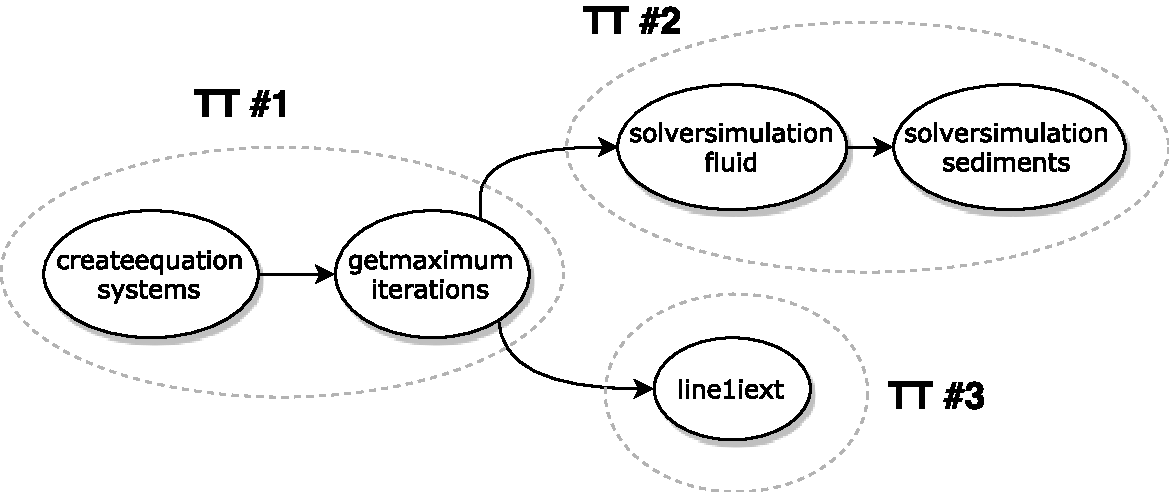
\includegraphics[width=\textwidth]{img/transformation-tracks}
    \caption[Exemplo de detecção das trilhas de transformações.]{Exemplo de detecção das trilhas de transformações de um fluxo de dados. Na figura existem três trilhas de transformações (\textsc{TT}).}%
    \label{fig:transformation-tracks}
\end{figure}

O algoritmo começa com as últimas transformações de \( D \) (encontradas no \autoref{lst:algorithm-last-transformations}), e caminha em direção às primeiras transformações de \( D \). A ideia principal é realizar a detecção do fim --- e, portanto, do início --- de cada trilha de transformação, que pode acontecer em várias situações: \textit{e.g.}, sempre que o grau de saída do vértide de transformação for maior do que 1, indicando que a transformação em questão possui várias transformações de saída.

\begin{minipage}[c]{0.95\textwidth}
\begin{lstlisting}[language=pseudocode,label={lst:algorithm-transformation-tracks},caption={[Detecção das trilhas de transformações]Detecção do rastro do fluxo de dados no nível de trilhas de transformações.}]
function getTransformationTracks(%\(D\)%):
    dtTracks %\leftarrow% {}
    lastDts %\leftarrow% getLastTransformations(%\(D\)%) %\quad%# %\autoref{lst:algorithm-last-transformations}%
    queue %\leftarrow% {}
    queue.push(lastDts)
    while queue is not empty do:
        dt %\leftarrow% queue.pop()
        nextDts %\leftarrow% getNextTransformations(%\(D\)%, dt)
        if lastDts.contains(dt)
           or hasManyOutputDatasets(%\(D\)%, dt)
           or hasManyNextTransformations(%\( D \)%, dt)
           or anyTransformationHasManyInputDatasets(%\(D\)%, nextDts)
           then:
            track %\leftarrow% new TransformationTrack()
            track.addTransformation(dt)
            dtTracks %\leftarrow% dtTracks + {track}
        else then:
            track %\leftarrow% getTransformationTrack(dtTracks, nextDts)
            track.addTransformation(dt)
        end if
        previousDts %\leftarrow% getPreviousTransformations(%\(D\)%, dt)
        queue.push(previousDts)
    end do
    return dtTracks
end function
\end{lstlisting}
\end{minipage}

A complexidade de tempo do algoritmo é linear da ordem de \( O(\#(T)) \), isto é, proporcional ao número de transformações de dados presentes em \( D \). As trilhas de transformações são armazenadas em listas encadeadas de transformações.

\subsection{Detecção das trilhas de conjuntos de dados}

O \autoref{lst:algorithm-dataset-tracks} tem como função obter as \textbf{trilhas de conjuntos de dados} \texttt{dsTracks} de um fluxo de dados \( D \). O conceito de trilha de conjuntos de dados é análogo ao de trilha de transformações de dados, mencionado na \autoref{subsec:deteccao-das-trilhas-de-transformacoes}: é uma forma de dividir e agrupar conjuntos de dados em diversos subconjuntos.

O algoritmo funciona com base no \autoref{lst:algorithm-transformation-tracks}: uma vez tomadas as trilhas de transformações de dados, é trivial obter cada uma das trilhas de conjuntos de dados a partir de cada uma delas. Para isso, basta tomar a união de todos os conjuntos de dados adjacentes (\textit{i.e.} anteriores e posteriores) a todas as transformações de dados de uma trilha de transformações.

\begin{minipage}[c]{0.95\textwidth}
\begin{lstlisting}[language=pseudocode,label={lst:algorithm-dataset-tracks},caption={[Detecção das trilhas de conjuntos de dados]Detecção do rastro do fluxo de dados no nível de trilhas de conjuntos de dados.}]
function getDatasetTracks(%\(D\)%):
    dsTracks %\leftarrow% {}
    dtTracks %\leftarrow% getTransformationTracks(D) %\quad%# %\autoref{lst:algorithm-transformation-tracks}%
    for each dtTrack %\in% dtTracks do:
        dsTrack %\leftarrow% {}
        for each dt %\in% dtTrack do:
            if dsTrack is empty then:
                nextDss %\leftarrow% getNextDatasets(%\(D\)%, dt)
                dsTrack %\leftarrow% dsTrack + {nextDss}
            end if
            previousDss %\leftarrow% getPreviousDatasets(%\(D\)%, dt)
            dsTrack %\leftarrow% dsTrack + {previousDss}
        end do
        dsTracks %\leftarrow% dsTracks + {dsTrack}
    end do
    return dsTracks
end function
\end{lstlisting}
\end{minipage}

A complexidade de tempo do algoritmo é a mesma do algoritmo do \autoref{lst:algorithm-transformation-tracks}: linear da ordem de \( O(\#(T)) \), e as trilhas de conjuntos de dados são também armazenadas em listas encadeadas de conjuntos de dados.

\subsection{Obtenção de múltiplos mapeamentos de atributos entre dois conjuntos de dados}

\perrotta{TODO: introduction with autoref, caption repeating + bold and algorithm explanation}

\begin{minipage}[c]{0.95\textwidth}
\begin{lstlisting}[language=pseudocode,label={lst:algorithm-attribute-mappings},caption={[Obtenção de múltiplos mapeamentos de atributos]Obtenção de múltiplos mapeamentos de atributos entre dois conjuntos de dados.}]
function getAttributesMapping(dt,%\(\textrm{ds}_{\textrm{input}}\)%,%\(\textrm{ds}_{\textrm{output}}\)%,type)
   attrs %\leftarrow% {}
   if type == physical then:
       attrs %\leftarrow% attrs + {t.getInstanceAttribute()}
   else:
       for each inAttr %\in% %\(\textrm{ds}_{\textrm{input}}\).A% do:
           for each outAttr %\in% %\(\textrm{ds}_{\textrm{output}}\).A% do:
               if inAttr.name == outAttr.name
                  and inAttr.type == outAttr.type then:
                   attrs %\leftarrow% attrs + {inAttr}
               end if
           end for
       end do
   end if
   %\mu% %\leftarrow% attributesMapping(attrs,dt,%\(\textrm{ds}_{\textrm{input}}\)%,%\(\textrm{ds}_{\textrm{output}}\)%)
   return %\mu%
end function
\end{lstlisting}
\end{minipage}

\perrotta{TODO: complexity and data structures}

\perrotta{TODO: Mais listings, com pseudocódigos, explicações e complexidade. Algoritmos de grafos (bfs/dfs) + query (como algoritmo 6)}
\perrotta{TODO: Mencionar o pré-processamento e as otimizações que fiz}
\perrotta{TODO: Como rodar --- explicar a assinatura da funcao principal}